\documentclass[10 pt]{article}
\usepackage{tikz}
\usetikzlibrary{arrows}
\usepackage[margin=0.5 in]{geometry}
\usepackage[utf8]{inputenc}
\usepackage{tabu}
\usepackage{color}
\usepackage{mathtools}
\usepackage{amsfonts}
\usepackage{xcolor}
\usepackage{listings}
\usepackage{enumitem}
\usepackage{multicol}
\setlength{\columnsep}{1cm} 
\newtheorem{theorem}{Teorema}
\usepackage{mathrsfs}
\title{\textbf {Estructuras de Datos y Algoritmos 1 - ST0245\\Segundo Parcial 002 - Martes}}
\author{Nombre ..............................\\
		Departamento de Informática y Sistemas\\
		Universidad EAFIT\\}
\date{Mayo 11 de 2021}
\begin{document}

\lstset{language=Java,frame=none, breaklines=true, numbers = left, stepnumber = 1, xleftmargin=5.0ex, showstringspaces=false, showspaces=false }
\lstset{language=Python,frame=none, breaklines=true, numbers = left, stepnumber = 1, xleftmargin=5.0ex, showstringspaces=false,showspaces=false }
\maketitle

\section{Árboles 30\%}
\begin{multicols}{2}
En empresas como Bancolombia, los árboles se utilizan para simbolizar decisiones; por ejemplo, las condiciones que se deben analizar para decidir
si a un cliente se le puede otorgar un crédito o no. Veamos un ejercicio interesante sobre árboles binarios --muy común en entrevistas según el portal
\emph{LeetCode}. 
Dado un árbol binario, es necesario encontrar el sub-árbol que tiene el mayor promedio. El promedio de un sub-árbol, es la suma del valor de su nodo raíz más la suma del valor de todos sus nodos descendientes, divido por el número de nodos que aportan a tal suma. Para el siguiente árbol, la respuesta es $9$ que corresponde al sub-árbol donde la raíz es el nodo $9$ y no tiene hijos ni izquierdo ni derecho. El siguiente código resuelve el problema, pero le faltan algunas líneas.

\begin{center}
    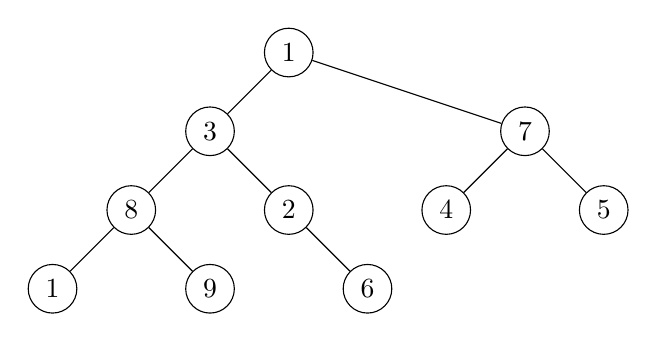
\begin{tikzpicture}
    
    \tikzset{vertex/.style = {shape=circle,draw,minimum size=1.5em}}
    \tikzset{edge/.style = {-,> = latex'}}
    \node[vertex] (G) at (0,0)  {1};
    \node[vertex] (I) at (3,-1)  {7};
    \node[vertex] (H) at (2,-2)  {4};
    \node[vertex] (J) at (4,-2)  {5};
    \node[vertex] (D) at (-1, -1) {3};
    \node[vertex] (E) at (0, -2) {2};
    \node[vertex] (F) at (1, -3) {6};
    \node[vertex] (B) at (-2, -2) {8};
    \node[vertex] (C) at (-1, -3) {9};
    \node[vertex] (A) at (-3, -3) {1};
    %edges
    \draw[edge] (G) to (D);
    \draw[edge] (D) to (B);
    \draw[edge] (D) to (E);
    \draw[edge] (E) to (F);
    \draw[edge] (B) to (A);
    \draw[edge] (B) to (C);
    \draw[edge] (G) to (I);
    \draw[edge] (I) to (H);
    \draw[edge] (I) to (J);
    \end{tikzpicture}
  \end{center}
\end{multicols}





\textbf{Si trabajas en Java}, considera el siguiente código:

{\small
\begin{lstlisting}[language=java]
class Node {
  Node left; Node right; int val;
  Node(int val) { this.val = val;
} } 

class Pair {
  int sum; int size;
  Pair(int sum, int size) {
    this.sum = sum; this.size = size;
} }

class Algorithm {
 static double promMax = 0.0;
 static double solve(Node root) {
  solveTemp(root); return promMax;
 }
 static Pair solveTemp(Node root) {
  if (root == null) return new Pair(0, 0);
  Pair l = solveTemp(root.left);
  Pair r = solveTemp(root.right);
  int sum = ......................;
  int sz = 1 + l.size + r.size;
  promMax = Math.max(promMax, .......................);
  return new Pair(sum, sz);
}}
\end{lstlisting}
}

\begin{enumerate}[label=(\Alph*)]
% Respuesta: l.sum + r.sum + root.val
\item (10\%) Completa la línea 21 .........................
% Respuesta: sum * 1.0 / sz
\item (10\%) Completa la línea 23 .........................
% Respuesta: T(n) = 2T(n/2) + c o T(n) = T(n-1) + c que, en ambos casos, es O(n)
\item (10\%) ¿Cuál es la ecuación de recurrencia, para el peor caso, del algoritmo anterior? T(n) = ...................
\end{enumerate}

\newpage

\textbf{Si trabajas en Python}, considera el siguiente código:

{\small
\begin{lstlisting}[language=python]
class Node:
  def __init__(self, val):
   self.val = val
   self.left = None
   self.right = None 

promMax = 0.0
theSum = 0
theSize = 1

def solve(root):
  solveTemp(root) 
  return promMax
 
def solveTemp(root):
  global promMax
  if root == None: 
     return (0, 0) #theSum, theSize
  l = solveTemp(root.left)
  r = solveTemp(root.right)
  sum = ......................
  sz = 1 + l[theSize] + r[theSize]
  promMax = max(promMax, .......................)
  return (sum, sz) #theSum, theSize

\end{lstlisting}
}

\begin{enumerate}[label=(\Alph*)]
% Respuesta: l[theSum] + r[theSum] + root.val o l[0] + r[0] + root.val
\item (10\%) Completa la línea 21 .........................
% Respuesta: sum * 1.0 / sz
\item (10\%) Completa la línea 23 .........................
% Respuesta: T(n) = 2T(n/2) + c o T(n) = T(n-1) + c que, en ambos casos, es O(n)
\item (10\%) ¿Cuál es la ecuación de recurrencia, para el peor caso, del algoritmo anterior? T(n) = ...................
\end{enumerate}

\newpage


\section{Pilas 20\%}



En la vida real, determinar si una cadena con paréntesis, llaves y corchetes es válida es de interés para grandes empresas como \emph{Microsoft} (creador del lenguaje C\#) u \emph{Oracle } (dueño del lenguaje Java). Además, es un ejercicio muy común en entrevistas para estas empresas según el portal \emph{Geeks for Geeks}. Veamos el problema. 
Dada una cadena que contiene --únicamente-- los caractéres ``('', ``\{'', ``['', ``)'', ``\}'', ``]'', determina si ésta es válida. La cadena es válida si para cada caractér que abre, siempre hay uno que cierra en el orden correcto. Como un ejemplo ``([ ])'' es válida, pero ``[({}])'' no es válida porque el paréntesis ``)'' debe cerrar antes que el corchete ``]''. ¡Sólo nos falta completar unas líneas! ¡Ánimo!

\hspace{1cm}

\textbf{Si trabajas en Java}, considera este código:

\begin{lstlisting}[language=Java]
boolean solve(String exp) {
  LinkedList<Character> s = new LinkedList();
  for(int i=0;i<exp.length();++i){
    char ei = exp.charAt(i);
    if(ei == '(' | ei == '{' | ei == '[')
      ..........................;
    if(ei == ')' | ei == '}' | ei == ']'){
      if(s.size() == 0 | !valid(s.get(s.size()-1), ei))
        return false;
      else{
        ..........................;
  } } }
  return s.size() == 0;
}
boolean valid(char o, char c) {
  return (o == '(' && c == ')') |
         (o == '[' && c == ']') |
         (o == '{' && c == '}');
}
\end{lstlisting}

En Java, la librería \texttt{LinkedList} se puede usar 
para implementar una pila. En esa librería, \texttt{push(e)}
agrega el elemento $e$ a la pila y \texttt{pop( )} elimina
el elemento que se encuenta en el tope de la pila.


\hspace{1cm}

\textbf{Si trabajas en Python}, considera este código:

\begin{lstlisting}[language=Python]
def solve(exp):
  s = deque()
  for i in range(0, len(exp)):
    ei = exp[i]
    if ei == "(" or ei == "{" or ei == "[":
      ..........................
    if ei == ")" or ei == "}" or ei == "]":
      if len(s) == 0 or not valid(s[len(s)-1], ei):
        return False
      else:
        ..........................
  return len(s) == 0

def valid(o, c):
  return (o == "(" and c == ")") or \
         (o == "[" and c == "]") or \
         (o == "{" and c == "}")
\end{lstlisting}

En Python, la librería \texttt{deque} se usa para implementar una pila. 
En \texttt{deque}, \texttt{append()} agrega al final y \texttt{pop()} elimina el último elemento.


\begin{enumerate}[label=(\Alph*)]
  % Solución: En Java: s.push(ei)  En Python: s.append(ei)
  \item (10\%) Completa la línea 6  ..............\\ \\
  % Solución: En Java: s.pop() o también s.remove(s.size()-1) y en Python: s.pop()
  Y Completa la línea 11 ..............
  % Solución: O(|e|)
  \item (10\%) Cuál es la complejidad asintótica, en el peor de los casos, del algoritmo anterior. \\ \\
  O(\line(1, 0){230}), donde $e$ es el número de caracteres de \texttt{exp}. NO existe $n$.
\end{enumerate}

\newpage





\section{Colas 20\%}
\begin{multicols}{2}
En la vida real, las colas circulares se usan para planificación de procesos en sistemas operativos como 
Microsoft Windows 10, Linux Ubuntu 21.04 y Mac OS X. Para lograrlo, se utilizan algoritmos como el de 
\textit{Round Robin} o versiones mejoradas de este algoritmo. Por ahora, vamos a limitarnos a implementar
una cola circular, que nos servirá mucho para trabajar en empresar como Microsoft, Redhat, Oracle o Apple.
Sólo nos falta una línea y la complejidad, ¿nos ayudas a completarlas? ¡Por favor! La imagen a continuación
muestra un ejemplo de una cola circular.



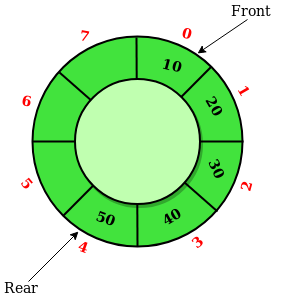
\includegraphics[width=0.23\textwidth]{Circular-queue.png}


\end{multicols}

\textbf{Si trabajas en Java}, considera este código:


\begin{lstlisting}[language = java]
public class CircularQueue {
    int[] queue; 
    int front;
    int rear; 
    int currentSize;
    int size;

    public CircularQueue(int size) { 
        this.queue = new int[size];
        this.front = 0;
        this.rear = 0;
        this.size = size;
        this.currentSize = 0;
    }
    public boolean add(int x) {
        if (currentSize == size) 
            throw new IllegalStateException("The queue is full: front size: " + rear); 
        queue[rear++] = x;
        .......................
        currentSize++;
        return true;
    }
    public int peek() {
        if (front == rear) 
            throw new IllegalStateException("The queue is empty");
        return queue[front];
    }
    public int poll() {
        if (front > rear) 
            throw new IllegalStateException("The queue is empty");
        currentSize--;
        return queue[front++];
}   }
\end{lstlisting}

En una cola circular, el método \texttt{add(e)} agrega un elemento al final de la cola (en inglés, \textit{rear})
el método \texttt{poll()} elimina el primer elemento que llegó a la cola (en inglés, \textit{front}) y el método
\texttt{peek()} permite ver el primer elemento que llegó a la cola, sin eliminarlo. El operador a \% b es el residuo de dividir $a$ en $b$.

\begin{enumerate}[label=(\Alph*)]
  % Solución: En Java : rear = (rear + 1) % size; 
  \item (10\%) Completa la línea 19  .....................
  % Solución: O(1)
  \item (10\%) Cuál es la complejidad asintótica, en el peor de los casos, del algoritmo anterior. \\ \\
  O(\line(1, 0){230}), donde $n$ es el número de elementos que hay en cola.
\end{enumerate}




\newpage


\textbf{Si trabajas en Python}, considera este código:


\begin{lstlisting}[language = python]
import numpy as np
class CircularQueue:
    def __init__(self, size): 
        self.queue = np.zeros(size)
        self.front = 0
        self.rear = 0
        self.size = size
        self.currentSize = 0
    
    def add(self, x):
        if self.currentSize == self.size: 
            raise Exception("The queue is full: front size: " + str(self.rear)) 
        self.queue[self.rear] = x
        self.rear += 1
        .......................
        self.currentSize += 1
        return True
    
    def peek(self):
        if self.front == self.rear: 
            raise Exception("The queue is empty");
        return self.queue[self.front]
    
    def poll(self):
        if self.front > self.rear: 
            raise Exception("The queue is empty");
        self.currentSize -= 1
        self.front += 1
        return self.queue[self.front-1]
\end{lstlisting}

En una cola circular, el método \texttt{add(e)} agrega un elemento al final de la cola (en inglés, \textit{rear})
el método \texttt{poll()} elimina el primer elemento que llegó a la cola (en inglés, \textit{front}) y el método
\texttt{peek()} permite ver el primer elemento que llegó a la cola, sin eliminarlo. El operador a \% b es el residuo de dividir $a$ en $b$.


\begin{enumerate}[label=(\Alph*)]
  % Solución:  En Python: self.rear = (self.rear + 1) % self.size
  \item (10\%) Completa la línea 15  .....................
  % Solución: O(1)
  \item (10\%) Cuál es la complejidad asintótica, en el peor de los casos, del algoritmo anterior. \\ \\
  O(\line(1, 0){230}), donde $n$ es el número de elementos que hay en cola.
\end{enumerate}


\newpage

\section{Tablas de Hash 20\%}
Cuando un sitio web te solicita tu login y password para autenticarte, el password que se almacena en el servidor es el hash del password. De esa manera, si un atacante accede a los passwords almacenados en el servidor, estos no le serán útiles para autenticarse en el sitio web. Consideremos otro problema con tablas de hash. 
Dada una cadena que contiene caracteres alfabéticos en minúsculas, tenemos que eliminar como máximo un carácter de esta cadena de manera que la frecuencia de cada carácter distinto sea la misma en la cadena. Sólo nos falta completar una línea y la complejidad, ayúdanos por favor.

\begin{multicols}{2}
\noindent
    \textbf{Entrada:} str = "xyyz" 

\noindent
    \textbf{Salida:} Sí 

\noindent
    Podemos eliminar el carácter 'y' de la cadena anterior cadena para que la frecuencia de cada carácter sea la misma. 

\noindent
    \textbf{Entrada:} str = "xyyzz" 

\noindent
    \textbf{Salida:} Sí 

\noindent
    Podemos eliminar el carácter 'x' de la cadena cadena para que la frecuencia de cada carácter sea la misma.

\noindent
    \textbf{Entrada:} str = "xxxxyyzz" 

\noindent
    \textbf{Salida:} No 

\noindent
    No es posible hacer que la frecuencia de cada carácter sea la misma simplemente eliminando como máximo un carácter de la cadena anterior.
\end{multicols}

\textbf{Si trabajas en Java}, considera este código:

{\small
\begin{lstlisting}
public class Hashing {
    static final int M = 26;
    static int getIdx(char ch) { // Metodo para obtener el indice de un caracter 
        return (ch - 'a');
    }
    // Retorna si todos los elementos del arreglo freq que ocurren mas de una vez son iguales
    static boolean allSame(int freq[], int N){
        int same = 0;
        int i; // Selecciona el primer elemento que ocurre mas de una vez
        for (i = 0; i < N; i++) {
            if (freq[i] > 0) {
                same = freq[i];
                break;
        }   }
        for (int j = i + 1; j < N; j++)
            if (freq[j] > 0 && freq[j] != same)
                return false;
        return true;
    }
    // Retorna verdadero si podemos hacer que todas las frecuencias sean iguales
    static boolean possibleSameCharFreqByOneRemoval(String str) {
        int l = str.length();        
        int[] freq = new int[M]; // Crea el arreglo de frecuencias 
        for (int i = 0; i < l; i++)
            freq[getIdx(str.charAt(i))]++;        
        if (allSame(freq, M)) // Si todas las frecuencias son iguales, 
            return true;      // retorna verdadero        
            int i = getIdx(c); //  Intenta bajar la frecuencia de cada caracter en uno             
            if (freq[i] > 0) { // Verifica si un caracter ocurre una sola vez en la cadena
                freq[i]--;
                if (allSame(freq, M))
                    return true;
                freq[i]++;
        }   }
        ...........................
}   }
\end{lstlisting}
}

\begin{enumerate}[label=(\Alph*)]
  % Respuesta: Java return false; Python return False
  \item (10\%) Completa la línea 35 ..........................
  % Respuesta: O(n)
  \item (10\%) ¿Cuál es la complejidad asintótica, para el peor de los casos, del último algoritmo? \\
  O(..........................) Donde $l$ es el número de elementos de la cadena. NO hay $n$ en este problema
\end{enumerate}

\newpage

\textbf{Si trabajas en Python}, considera este código:

{\small
\begin{lstlisting}
M = 26
# Funcion para obtener el indice de un caracter 
def getIdx(ch):
    return (ord(ch) - ord('a')) 
# Retorna si todos los elementos del arreglo freq que ocurren mas de una vez son iguales
def allSame(freq, N):    
    # Selecciona el primer elemento que ocurre mas de una vez
    for i in range(0, N):
        if(freq[i] > 0):
            same = freq[i]
            break   
    for j in range(i + 1, N):
        if(freq[j] > 0 and freq[j] != same):
            return False
    return True
# Retorna verdadero si podemos hacer que todas las frecuencias sean iguales
def possibleSameCharFreqByOneRemoval(str1):
    l = len(str1)
    # Crea el arreglo de frecuencias 
    freq = [0] * M
    for i in range(0, l):
        freq[getIdx(str1[i])] += 1    
    # Si todas las frecuencias son iguales, retorna verdadero
    if(allSame(freq, M)):
        return True
     
    # Intenta bajar la frecuencia de cada caracter en uno  
    for i in range(0, 26):
        # Verifica si un caracter ocurre una sola vez en la cadena
        if(freq[i] > 0):
            freq[i] -= 1
            if(allSame(freq, M)):
                return True
            freq[i] += 1
    .................
\end{lstlisting}
}

\begin{enumerate}[label=(\Alph*)]
  % Respuesta: Java return false; Python return False
  \item (10\%) Completa la línea 35 ..........................
  % Respuesta: O(n)
  \item (10\%) ¿Cuál es la complejidad asintótica, para el peor de los casos, del último algoritmo? \\
  O(..........................) Donde $l$ es el número de elementos de la cadena. NO hay $n$ en este problema
\end{enumerate}


\newpage


\section{Grafos 10\%}

  El coloramiento de grafos es un problema fundamental en la ingeniería de sistemas y matemática: A partir de este problema se pueden resolver muchas tareas, como lo son asignación de salones, de jaulas en zoológicos, de semáforos o colorear un mapa. Por eso, hoy vamos a desarrollar un algoritmo para colorear un grafo con la mínima cantidad de colores que, infortunadamente, no siempre entrega la mínima cantidad de colores por ser ávaro. Ayúdanos a resolver el problema de encontrar la mínima cantidad de colores para pintar un grafo cualquiera. Colorear un grafo quiere decir asignar colores a sus vértices de tal forma que dos vértices adyacentes  NO queden con el mismo color. El algoritmo y un ejemplo están a continuación.

  \begin{multicols}{2}

  \begin{itemize}[noitemsep]
    \item Colorear el vértice $0$ con el color $0$.
    \item Por cada uno de los restantes $n – 1$ vertices del grafo, 
    \begin{itemize}
     \item Tomar un vértice $u$. 
     \item Colorear $u$ con el menor color que aún no ha sido utilizado para colorear sus vértices adyacentes. 
     \item Si todos los colores previos ya han sido utilizados, colorear $u$ con un nuevo color.
    \end{itemize}
  \end{itemize}

  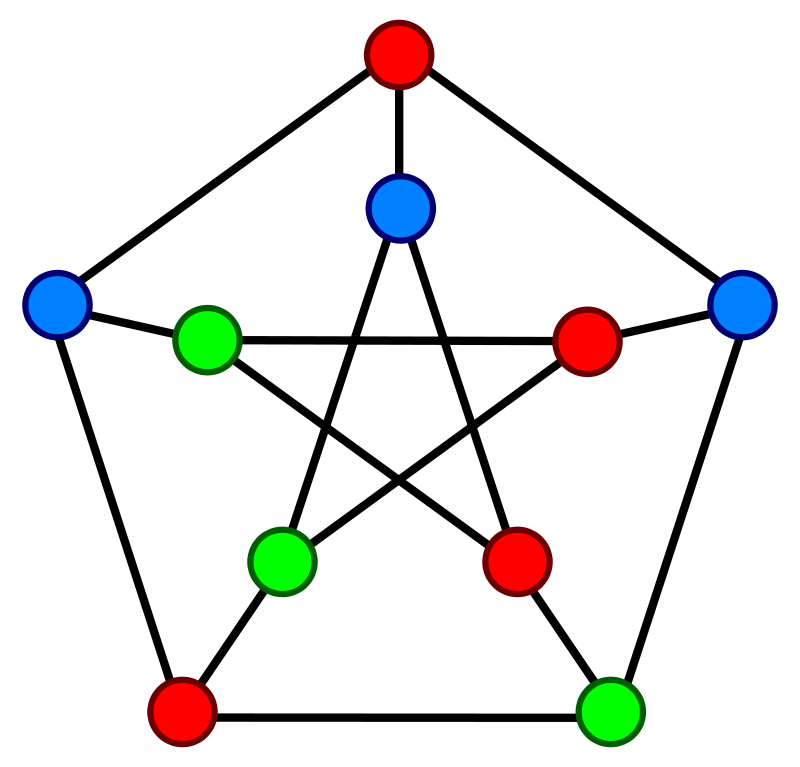
\includegraphics[width=0.18\textwidth]{coloring.png}

\end{multicols}

\textbf{Si trabajas en Java}, considera este código:

  \begin{lstlisting}[language = java]
int colorear(boolean[][] grafo) {
    int n = grafo.length;
    int[] color = new int[n + 1];
    for(int i = 0; i < n; ++i) 
      color[i] = -1;
    color[0] = 0;
    boolean[] colordisponible = new boolean[n + 1];
    for(int i = 0; i < n; ++i) 
      colordisponible[i] = true;
    for(int u = 1; u < n; ++u) {
      for(int i = 0; i < n; ++i)
        if(grafo[u][i])
          if(color[i] != -1)
            colordisponible[color[i]] = false;
      int aval;
      for(aval = 0; aval < n; ++aval)
       if(colordisponible[aval])
         break;
      color[u] = aval; 
    }
    for(int i = 0; i < n; ++i) 
      colordisponible[i] = true;
    boolean[] usado = new boolean[n + 1];
    int res = 0;
    for(int i = 0; i < n; ++i) 
      if(!usado[color[i]]){
        usado[color[i]] = true; 
        res++;
      }
    return res+1;
}
  \end{lstlisting}




  \begin{enumerate}[label=(\Alph*)]
    % O(V ^ 2)
    \item (10\%) ¿Cuál es la complejidad asintótica, en el peor de los casos, del algoritmo anterior? Donde $V$ es el número de vértices del grafo.
    \begin{enumerate}[label=\roman*)]
      \item $O(V)$
      \item $O(V \times \log(V))$
      \item $O(V^2)$
      \item $O(1)$
      \item $O(V^3)$
      \item $O(\log(V))$
    \end{enumerate}
  \end{enumerate}



\newpage

\textbf{Si trabajas en Python}, considera este código:


\begin{lstlisting}[language = python]
def colorear(grafo):
    n = len(grafo)
    color = np.zeros(n+1)
    for i in range(0,n):
      color[i] = -1
    color[0] = 0
    colordisponible = np.zeros(n + 1)
    for i in range(0,n):
      colordisponible[i] = 1
    for u in range (1,n):
      for i in range(0,n):
        if grafo[u][i] == 1:
          if color[i] != -1:
            colordisponible[int(color[i])] = 0
      color[u] = 0
      for aval in range(0,n):
       if colordisponible[aval] == 1:
         color[u] = aval
         break     
    for i in range(0,n):
      colordisponible[i] = 1
    usado = np.zeros(n+1)
    res = 0
    for i in range(0,n):
      if usado[int(color[i])] == 0:
        usado[int(color[i])] = 1 
        res = res +1
    return res+1
  \end{lstlisting}
  \begin{enumerate}[label=(\Alph*)]
    % O(V^2)
    \item (10\%) ¿Cuál es la complejidad asintótica, en el peor de los casos, del algoritmo anterior? Donde $V$ es el número de vértices del grafo.
    \begin{enumerate}[label=\roman*)]
      \item $O(V)$
      \item $O(V \times \log(V))$
      \item $O(V^2)$
      \item $O(1)$
      \item $O(V^3)$
      \item $O(\log(V))$
    \end{enumerate}
  \end{enumerate}


\newpage

\section{Meme sobre Complejidad (2\% extra)}
 (2 \%)  En la vida real, los memes se utilizan en presentaciones orales como una estrategia para \textit{romper el hielo}. Con base en los errores que has cometido durante el semestre sobre complejidad, 
escribe un texto para el siguiente meme:\\
................................................     ................................................\\
................................................     ................................................\\
................................................     ................................................\\
................................................     ................................................\\
................................................     ................................................\\
................................................     ................................................\\
................................................     ................................................\\

\includegraphics[width=0.5\textwidth]{Meme.jpg}


Como un ejemplo, ten en cuenta la regla de la suma, regla del producto,
notación O o ecuaciones de recurrencia.



\newpage


\section{(Opcional) Árboles 10\%}
\begin{multicols}{2}
En la vida real, en arquitecturas de red para sistemas con memoria distribuida, es de suma importancia el diámetro de un árbol. 
Como bien sabes, un \emph{árbol} es un grafo no dirigido con $n$ vértices y $n - 1$ artistas donde el peso de cada arista es 1. Considera un árbol $g$ con raíz $v$. Sabemos que $d_i$, usando algoritmo de \emph{búsqueda primero en amplitud} (en Inglés, BFS), es la distancia más corta  del nodo $v$ al nodo $i$. En este ejercicio, vamos a encontrar el \textit{diámetro} de un árbol de $n$ nodos. El diámetro de un árbol se define como el número máximo de aristas del camino más corto entre cualesquiera dos vértices del árbol. Como un ejemplo, en el siguiente árbol, se resalta su diámetro, el cual es de longitud $4$. Como un árbol es un grafo, en este ejercicio, el árbol se representa como un grafo utilizando listas de adyacencia. 
  \\
  \begin{center}
    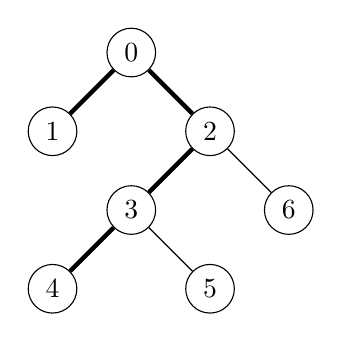
\begin{tikzpicture} 
    \tikzset{vertex/.style = {shape=circle,draw,minimum size=1.5em}}
    \tikzset{edge/.style = {-,> = latex'}}
    \node[vertex] (0) at (0, 0)  {0};
    \node[vertex] (1) at (-1, -1) {1};
    \node[vertex] (2) at (1, -1) {2};
    \node[vertex] (3) at (0, -2) {3};
    \node[vertex] (4) at (-1, -3) {4};
    \node[vertex] (5) at (1, -3) {5};
    \node[vertex] (6) at (2, -2) {6};
    %edges
    \draw[-, ultra thick] (0) to (1);
    \draw[-, ultra thick] (0) to (2);
    \draw[-, ultra thick] (2) to (3);
    \draw[-, ultra thick] (3) to (4);
    \draw[edge] (3) to (5);
    \draw[edge] (2) to (6);
    \end{tikzpicture}
  \end{center}

\end{multicols}


\textbf{Si trabajas en Java}, considera este código:

\hspace{1cm}

La siguiente es la implementación del algoritmo de BFS para calcular las
  distancias más cortas del nodo $v$ a todos los demás nodos de un árbol
  {\footnotesize
  \begin{lstlisting}
  //Retorna di: las distancias mas cortas del nodo v al nodo i
  int[] bfs(ArrayList<Integer>[] g, int v) {
    int[] d = new int[g.length];
    Arrays.fill(d, Integer.MAX_VALUE);
    d[v] = 0;
    Queue<Integer> q;
    q = new LinkedList<Integer>();
    q.add(v);
    while(!q.isEmpty()){
      int s = q.poll();
      Iterator<Integer> i=g[s].listIterator();
      while(i.hasNext()){
        int n = i.next();
        if(d[s] + 1 < d[n]){
          d[n] = d[s] + 1;
          q.add(n);
    } } }
    return d;
  }
  \end{lstlisting}
  }
 {\footnotesize
  Para encontrar el diámetro de un árbol se puede usar el siguiente algoritmo:
  \begin{itemize}[noitemsep]
    \item Tomar un vértice $v$ como raíz del árbol $g$ y encontrar $d_i$, para todo $i$, usando \texttt{bfs(g, v)}.
    \item Encontrar un vértice $u$ como nodo inicial tal que $d_u \geq d_t$ para todo $t$. Sea $f_i$ la distancia más corta del nodo $u$ a cualquier nodo $i$ del árbol, el diámetro del árbol es $\max\limits_i{f_i}$
  \end{itemize}
 
  \begin{lstlisting}
  int diametro(ArrayList<Integer> g[]){
    int v, u, w;
    v = u = w = 0;
    int[] d = bfs(g, v);
    int n = d.length;
    for(int i = 0; i < n; ++i)
      if( ............ ) u = i;
    int[] f = bfs(g, u);
    for(int i = 0; i < n; ++i)
      if( .......... ) w = i;
    return f[w];
  }
  \end{lstlisting}
  }
  \begin{enumerate}[label=(\Alph*)]
    \item (10\%) ¿Cuál es la complejidad asintótica, en el peor de los casos, del algoritmo anterior? Donde $n$ es el número de vértices del árbol.
    % Respuesta O(n)
    \begin{enumerate}[label=\roman*]
      \item $O(\log_2 n)$
      \item $O(n)$
      \item $O(n^2)$
      \item $O(n \log_2 n)$
      \item $O(n \times \sqrt{n})$
    \end{enumerate}
    % Respuesta: d[i] > d[u], f[i] > f[w]
    Y Completa las líneas 7, 10 ............, ............
  \end{enumerate}

\newpage



\textbf{Si trabajas en Python}, considera este código:

\hspace{1cm}

La siguiente es la implementación del algoritmo de BFS para calcular las
  distancias más cortas del nodo $v$ a todos los demás nodos de un árbol
  {\footnotesize
  \begin{lstlisting}
#Retorna di: las distancias mas cortas del nodo v al nodo i
def bfs(g,  v):
    # Rellena un arreglo con "infinito" con el num vertices de g
    d = np.full(len(g), np.iinfo(np.int32).max)
    d[v] = 0
    q = deque()
    q.append(v)
    while(len(q) != 0):
      s = q.pop()
      for n in g[s]:        
        if d[s] + 1 < d[n]:
          d[n] = d[s] + 1
          q.append(n)
    return d
  \end{lstlisting}
  }

  Para encontrar el diámetro de un árbol se puede usar el siguiente algoritmo:
  \begin{itemize}[noitemsep]
    \item Tomar un vértice $v$ como raíz del árbol $g$ y encontrar $d_i$, para todo $i$, usando \texttt{bfs(g, v)}.
    \item Encontrar un vértice $u$ como nodo inicial tal que $d_u \geq d_t$ para todo $t$. Sea $f_i$ la distancia más corta del nodo $u$ a cualquier nodo $i$ del árbol, el diámetro del árbol es $\max\limits_i{f_i}$
  \end{itemize}
  {\footnotesize
  \begin{lstlisting}
def diametro(g):
    v = u = w = 0
    d = bfs(g, v)
    n = d.size
    for i in range(0,n):
      if ............ :
          u = i
    f = bfs(g, u)
    for i in range (0,n):
      if .......... :
          w = i
    return f[w]
  \end{lstlisting}
  }
  \begin{enumerate}[label=(\Alph*)]
    \item (10\%) ¿Cuál es la complejidad asintótica, en el peor de los casos, del algoritmo anterior? Donde $n$ es el número de vértices del árbol.
    % Respuesta O(n)
    \begin{enumerate}[label=\roman*]
      \item $O(\log_2 n)$
      \item $O(n)$
      \item $O(n^2)$
      \item $O(n \log_2 n)$
      \item $O(n \times \sqrt{n})$
    \end{enumerate}
    % Respuesta: d[i] > d[u], f[i] > f[w]
    Y Completa las líneas 6, 10 ............, ............
  \end{enumerate}



\end{document}